\label{chap:virtualKeyboard}
As mentioned in section \ref{obj2}, one of the goals of this project is to provide the system with a way of accepting keyboard input from the user. This is in service of creating peripherals for the operating system to manage. It also provides a convenient way of demonstrating the thread management system as in real operating systems threads will often suspend themselves waiting for input.
\subsection{UI design}
The keyboard was based of my real world keyboard. Due to this many of the keys are more decorative than practical as they do not all have an ASCII \cite{ascii} equivalent. The layout was designed in glade \cite{glade} and saved as a XML file which could be loaded by a python script. Glade was a helpful tool to perform some of the less technical work for this section. The glade editor provided an easy way of laying out the keyboard on a grid, a specifying an ID for each button. 


\begin{figure}[ht!]
	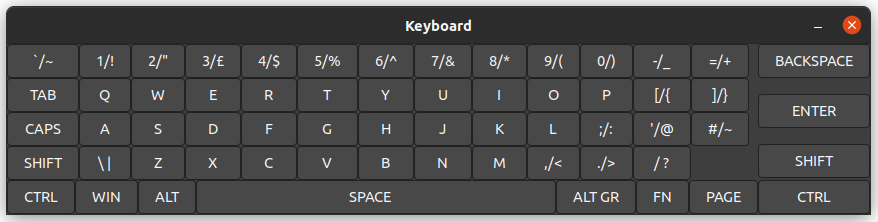
\includegraphics[width=\linewidth]{figures/keyboard.png}
	\caption{The final design of the virtual keyboard.}
	\label{fig:keyboard}
\end{figure} 




\subsection{Implementation}
\subsubsection{Python Script}
The virtual keyboard is implemented as a python \cite{python} script which runs in a separate process forked by Jimulator at runtime. This script simply loads the XML file produced by glade and runs the window seen by the user. It then continuously loops, checking for any change in state of the buttons. It can then use this data to report any state changes.  These state changes are written to a block of shared memory created in this python script. The Jimulator plug-in reads this shared memory and writes it to an interface in komodo's memory.
\subsubsection{Jimulator Plug-in Integration}
The Jimulator Plug-in is called by on Komodo loading. This C++ plug-in \cite{cbook} forks and executes the python script. It then attaches the shared memory in the python script to allow for communication between the glade application and Komodo. This plug-in then creates the interface between the ARM code running and the data generated by the glade keyboard. The interface is formed of 3 main registers assigned statically in the ARM chips memory. The first two registers are for transmitting the ASCII key pushed and the direction of the push (Up or Down). The third register is written two by the Operating System to acknowledge the key-press and free up the registers for new data. On a key push, plug-in will throw an interrupt and load the key data and key direction data into the correct registers. The Operating System will respond to the interrupt by reading the data, passing it to an application and clearing the interrupt via the interfaces acknowledge register. The specifics of passing the data to the application depend on the application method of querying the keyboard. There are two methods, `polling` and `interrupt based`. For both of these methods the plug-in works in the exact same way, the only difference is how to application code reads the data. When an interrupt is thrown and handled, by the keyboard, the data is written to a map in the Operating System's memory. The application can then either choose polling, in which the application continuously reads this map until a key-press is found, or it can choose the interrupt based method, in which the thread running the application suspends itself pending the keyboards next interrupt. When this interrupt is seen the application code reads the map which will have a key press in it and then returns to execution. This process is described in depth in section \ref{chap:Threading}.
\begin{figure}[ht!]
	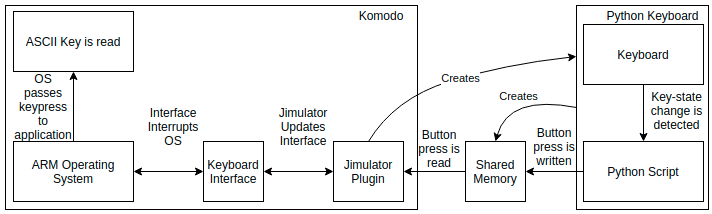
\includegraphics[width=\linewidth]{figures/jimulator.png}
	\caption{The full integration of the virtual keyboard with Komodo.}
	\label{fig:keyboard_integration}
\end{figure} 
\subsubsection{The Keyboard Interface In Komodo}
I have worked with the interface described in figure \ref{fig:keypad} before, so when developing a new interface I took what I learnt from using this. The described interface is efficient in terms of space complexity, however this results in a much larger burden on the software required to poll it. Polling this keypad requires the system to activate the individual scan-lines located in bits 7, 6 and 5, and read the output. This would take a long time with a device as large as my keyboard, and the problem is further complicated by the arrangement of my keys, as they do not conform to an \verb|n x m| grid like the keypad does. Therefore, I chose that the interface should consist of the three 32 bit registers to return the data. 


\subsection{Reverse Engineering The Jimulator Plug-in}
I had to develop the Jimulator Plug-in with only the source code of a few other plug-ins to use as a reference. While these plug-ins were effective for developing the functionality required to connect shared memory and fork processes, they didn't explain the minutiae of how to implement the functions Jimulator required. From reading these plug-ins I could determine that I needed to implement the following functions:
\begin{lstlisting}[
	style = myListingStyle,
	caption = {Jimulator functions}
	]
boolean constructor(unsigned char *name, unsigned char *arguments)
boolean destructor(unsigned char *name)
void irq_handler(uint8_t *irq, uint8_t *fiq)
boolean mem_r_handler(uint address, uint *data, int size, boolean sign, boolean T, int source, boolean* abort)
boolean mem_w_handler(uint address, uint data, int size, boolean T, int source, boolean* abort)
\end{lstlisting}

Of these functions, the most critical to understand were the \verb|mem_r_handler|, \verb|mem_w_handler| and \verb|irq_handler|. From my testing, I determined that these are called each clock cycle. In addition I determined that they should return a boolean value representing whether the function had handled the call on the parameters. For example, if I made a valid read to my keyboard interface, the \verb|mem_r_handler| would return a \verb|True| whereas a read to random address in memory should return a \verb|False|. The functions also needed to update the abort pointer with a boolean value, determining whether to signal the emulator to trigger an abort. This would have the usual effect of a data abort in ARM, it would switch mode to abort mode, and maintain the failing operation address in the LR.



\subsection{Evaluation and Improvements}
The keyboard does accomplish Objective 2 to some degree of success. It does reliably dispatch keys to the Operating system to handle. However, there are some minor improvement which I would have liked to have made. For example, this keyboard contains a single buffered item. Most modern keyboards have a larger buffer so that it is possible to queue up keys in the buffer. This ensures that the Operating system does not miss keys due to a full buffer. My current implementation will grab the first key and then not be able to read more items due to the full buffer. This makes the prompt reading of the buffer critical as keystrokes are often followed by the key being released. Clearly this is a rather significant flaw, however it does not detract from my original goal for the keyboard which was to give the operating system some IO to manage, and some reasons to suspend threads. The keyboard does actually function relatively well as a keyboard despite the small buffer due to the fact that its is a virtual keyboard only accessible by clicking. This means its quite hard to `type` fast, so in reality the buffer issue doesn't impact its effectiveness as much as you might think. The keyboard is also able to recognise capital letters via the use of the caps-lock button as well as grammar characters and what I refer to as control characters. The control characters are the keys I used to implement the ASCII characters backspace, horizontal tabulate, line feed, and carriage return. This was one of the more difficult features to implement as it these characters require special handling.
A further improvement I could make to the keep board is the ability to recognise and report combined key presses like \verb|ctrl-A|. This would require a large rework of how glade reports the key presses, but it would not be impossible. 